\documentclass[11pt]{article}

\usepackage{setspace}
\usepackage[margin=1in]{geometry}
\usepackage{graphicx}
% \usepackage{amsmath}
\usepackage{mathtools}
\usepackage{natbib} %for citet and citep
\usepackage{syntonly}
\usepackage{esdiff} %for writing partial derivatives
\usepackage{url} %for inserting urls
\usepackage{placeins}
\usepackage{textcomp} % for tildas
% \syntaxonly for quickly checking document
%set document settings

 \doublespacing % from package setspacs

% table font size
\let\oldtabular\tabular
\renewcommand{\tabular}{\scriptsize\oldtabular}

\title{A Bayesian wind farm investment model with an option of waiting}

\author{Jostein Lillest\o l & Johannes Mauritzen\\
 		Department of Business and Management Science\\
   NHH Norwegian School of Economics\\
   Bergen, Norway\\
%   johannes.mauritzen@nhh.no\\
%   \url{jmaurit.github.io}\\
		}
\date{\today}


\begin{document}

\begin{spacing}{1} %sets spacing to single for title page

\maketitle

\begin{abstract}
 ...
\end{abstract}

\thanks{*We would like to thank Endre Bj\o rndal, Jonas Andersson, and Gunnar Eskeland for helpful comments and suggestions. Data has been generously provided by Kjeller Vindteknikk. Financial support has been received from the Research Council of Norway through the projects INTREPID and CenSES.}
%JEL Codes: Q4, L71
\end{spacing}

\section{Introduction}

Unlike traditional energy generation technologies, the efficiency and profitability of wind turbines and wind farms are highly dependent on their location. Even modest differences in long-term average wind speeds can have major consequences on the profitability of wind farms over time. However, the inherent appropriateness of a given location is subject to high degree of uncertainty as wind speeds can vary substantially even within areas where overall wind resources are good. More so, average wind speeds show a high degree of variance from month-to-month and even year-to-year.

The high degree of spatial uncertainty of wind speeds leads to large uncertainty when making wind farm investment decisions. In this article we propose a simple sequential Bayesian decision model that takes into account spatial uncertainty and allows for the option of waiting to collect more information on wind speeds.

We first introduce a simple two period toy model with linear loss function. This simple model can be solved analytically, generating some stylized results that provide intuition and a frameworks for interpreting more complicated models. 

We then introduce a more realistic case study with data from a proposed wind farm in Northern Norway. We introduce realistic wind turbine power output function and investment loss functions that reflect the real-life non-linear relationship between wind-speeds and power generation. We use the Bayesian posterior sampling and modeling language Stan \ref{Stan} to simulate sampling from the posterior. This approach allows the model to be easily extended to take into account, for example, price and regulatory uncertainty.   


\section{Analytic Frameworks}


\section{Case Study: The Andmyran Wind Farm in Northern Norway}

We consider the case of the proposed Andmyran wind farm, located on an island in northern Norway. To establish the basis for the prior beliefs about the wind resources of the given location, we gather publicly available information on average wind speeds from three nearby weather stations: Andenes, Harstad and Sortland. This is obtained from the website of the Norwegian Meteorological Society's public weather page, \url{yr.no}. 

Figure \ref{avg_wind_speed_data} shows a chart of the average monthly wind speeds for the three sites. We can note the significant variation in average wind speed between the sites, even though they are all within 50 kilometers of one another. 

\begin{figure}
	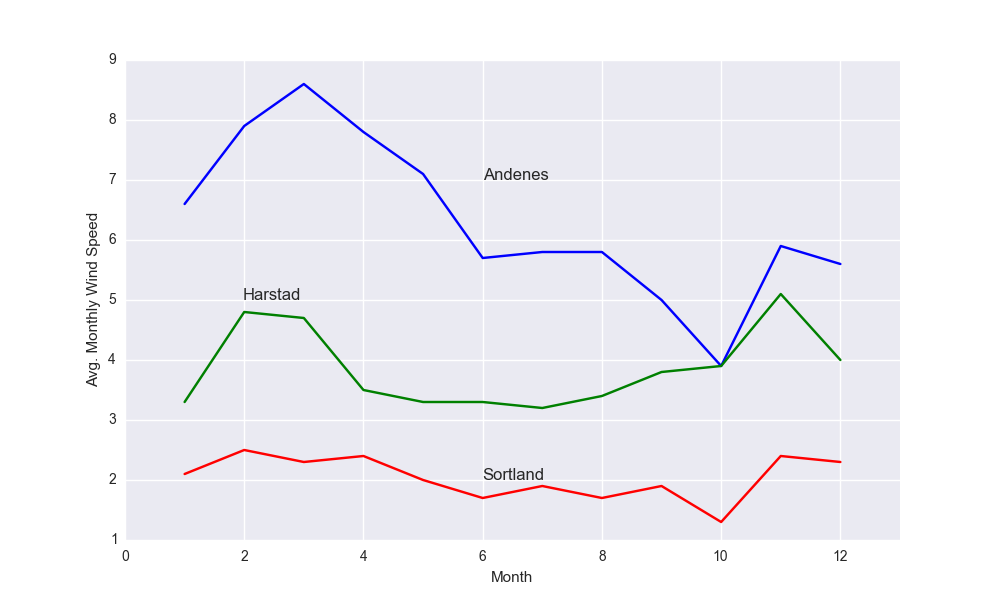
\includegraphics[width=1\textwidth]{figures/avg_wind_speed_data.png}
	\caption{Average monthly wind speeds from the three closest weather stations to the proposed Andymren site.}
	\label{avg_wind_speed_data}
\end{figure}

Wind speeds measured at shorter intervals are known to roughly follow a weibull distribution \footnote{A weibull distribution is defined has having a probability distribution function of $f(x, \lambda, k) = \frac{k}{\lambda} \frac{x}{\lambda}^{k-1} e^{-\frac{x}{\lambda}^k}$}. Thus we use the formula for the mean of a weibull distribution, as shown in equation \ref{mean_weibull}. Here $Gamma$ represents the Gamma function.

\begin{equation}
\mu_{weibull} = k*Gamma(1+\frac{1}{\lambda})^2
\label{mean_weibull}
\end{equation}

A simple least-squares optimisation routine is run in order to choose point estimates for the $k$ and $\lambda$ values of a weibull distribution that represents the prior uncertainty of wind speeds in the general area.



\end{document}


